\chapter{Automated planning}


\section{Definitions}

\begin{description}
    \item[Automated planning] \marginnote{Automated planning} 
        Given:
        \begin{itemize}
            \item An initial state.
            \item A set of actions an agent can perform (operators).
            \item The goal to achieve.
        \end{itemize}
        Automated planning finds a partially or totally ordered set of actions
        that leads an agent from the initial state to the goal.

    \item[Domain theory] \marginnote{Domain theory}
        Formal description of the executable actions.
        Each action has a name, pre-conditions and post-conditions.
        \begin{descriptionlist}
            \item[Pre-conditions] 
                Conditions that must hold for the action to be executable.
            \item[Post-conditions] 
                Effects of the action.
        \end{descriptionlist}

    \item[Planner] \marginnote{Planner}
        Process to decide the actions that solve a planning problem.
        In this phase, actions are considered:
        \begin{descriptionlist}
            \item[Non decomposable] 
                An action is atomic (it starts and finishes).
                Actions interact with each other by reaching sub-goals.
            \item[Reversible] 
                Choices are backtrackable.
        \end{descriptionlist}

        A planner can have the following properties:
        \begin{descriptionlist}
            \item[Correctness] \marginnote{Correct planner}
                The planner always finds a solution that leads from the initial state to the goal.
            \item[Completeness] \marginnote{Complete planner}
                The planner always finds a plan when it exists (planning is semi-decidable).
        \end{descriptionlist}

    \item[Execution] \marginnote{Execution}
        The execution is the implementation of a plan. 
        In this phase, actions are:
        \begin{descriptionlist}
            \item[Irreversible]
                An action that has been executed cannot (usually) be backtracked.
            \item[Non deterministic] 
                An action applied to the real world may have unexpected effects due to uncertainty.
        \end{descriptionlist}

    \item[Generative planning] \marginnote{Generative planning}
        Offline planning that creates the entire plan before execution based on
        a snapshot of the current state of the world.
        It relies on the following assumptions:
        \begin{descriptionlist}
            \item[Atomic time] 
                Actions cannot be interrupted.
            \item[Determinism] 
                Actions are deterministic.
            \item[Closed world] 
                The initial state is fully known, 
                what is not in the initial state is considered false (which is different from unknown).
            \item[No interference] Only the execution of the plan changes the state of the world.
        \end{descriptionlist}
\end{description}



\section{Linear planning}
\marginnote{Linear planning}
Formulates the planning problem as a search problem where:
\begin{itemize}
    \item Nodes contain the state of the world.
    \item Edges represent possible actions.
\end{itemize}
Produces a totally ordered list of actions.

The direction of the search can be:
\begin{descriptionlist}
    \item[Forward] \marginnote{Forward search}
        Starting from the initial state, the search terminates when a state containing a superset of the goal is reached.
    \item[Backward] \marginnote{Backward search}
        Starting from the goal, the search terminates when a state containing a subset of the initial state is reached.

        Goal regression is used to reduce the goal into sub-goals.
        Given a (sub-)goal $G$ and a rule (action) $R$ with delete-list (states that are false after the action) \texttt{d\_list}
        and add-list (states that are true after the action) \texttt{a\_list}, regression of $G$ through $R$ is defined as:
        \[
            \begin{split}
                \texttt{regr[$G$, $R$]} &= \texttt{true} \text{ if } G \in \texttt{a\_list} \text{ (i.e. regression possible)} \\
                \texttt{regr[$G$, $R$]} &= \texttt{false} \text{ if } G \in \texttt{d\_list} \text{ (i.e. regression not possible)} \\
                \texttt{regr[$G$, $R$]} &= G \text{ otherwise} \text{ (i.e. $R$ does not influence $G$)} \\
            \end{split}  
        \]

        \begin{example}[Moving blocks]
            Given the action \texttt{UNSTACK(X, Y)} with:
            \[
                \begin{split}
                    \texttt{d\_list} &= \{ \texttt{handempty}, \texttt{on(X, Y)}, \texttt{clear(X)} \} \\
                    \texttt{a\_list} &= \{ \texttt{holding(X)}, \texttt{clear(Y)} \}
                \end{split}
            \]
            We have that:
            \[
                \begin{split}
                    \texttt{regr[holding(b), UNSTACK(b, Y)]} &= \texttt{true} \\
                    \texttt{regr[handempty, UNSTACK(X, Y)]}  &= \texttt{false} \\
                    \texttt{regr[ontable(c), UNSTACK(X, Y)]} &= \texttt{ontable(c)} \\
                    \texttt{regr[clear(c), UNSTACK(X, Y)]} &= \begin{cases}
                        \texttt{true} & \text{if \texttt{Y}=\texttt{c}} \\
                        \texttt{clear(c)} & \text{otherwise}
                    \end{cases}
                \end{split}  
            \]
        \end{example}
\end{descriptionlist}


\subsection{Deductive planning}
\marginnote{Deductive planning}
Formulates the planning problem using first-order logic to represent states, goals and actions.
Plans are generated as theorem proofs.

\subsubsection{Green's formulation}
\marginnote{Green's formulation}
Green's formulation is based on \textbf{situation calculus}.
To find a plan, the goal is negated and it is proven that it leads to an inconsistency.

The main concepts are:
\begin{descriptionlist}
    \item[Situation]
        Properties (fluents) that hold in a given state \texttt{s}.
        \begin{example}[Moving blocks]
            To denote that \texttt{ontable(c)} holds in a state \texttt{s}, we use the axiom:
            \[ \texttt{ontable(c, s)} \]
        \end{example}
        The operator \texttt{do} allows to evolve the state such that:
        \[ \texttt{do(A, S)} = \texttt{S'} \]
        \texttt{S'} is the new state obtained by applying the action \texttt{A} in the state \texttt{S}.

    \item[Actions]
        Define the pre-condition and post-condition fluents of an action in the form:
        \[ \texttt{pre-conditions} \rightarrow \texttt{post-conditions} \]
        Applying the equivalence $A \rightarrow B \equiv \lnot A \vee B$, actions can be described by means of disjunctions.
        \begin{example}[Moving blocks]
            The action \texttt{STACK(X, Y)} has pre-conditions \texttt{holding(X)} and \texttt{clear(Y)}, and
            post-conditions \texttt{on(X, Y)}, \texttt{clear(X)} and \texttt{handfree}.
            Its representation in Green's formulation is:
            \[
                \begin{split}
                    \texttt{holding(X, S)} \land \texttt{clear(Y, S)} &\rightarrow \\
                    &\texttt{on(X, Y, do(STACK(X, Y), s))} \land \\
                    &\texttt{clear(X, do(STACK(X, Y), s))} \land \\
                    &\texttt{handfree(do(STACK(X, Y), s))} \\
                \end{split}
            \]
        \end{example}

    \item[Frame axioms]
        Besides the effects of actions, each state also has to define for all non-changing fluents their frame axioms.
        If the problem is complex, the number of frame axioms becomes unreasonable.
        \begin{example}[Moving blocks]
            \[ \texttt{on(U, V, S)} \land \texttt{diff(U, X)} \rightarrow \texttt{on(U, V, do(MOVE(X, Y, Z), S))} \]
        \end{example}
\end{descriptionlist}


\begin{example}[Moving blocks]
    The initial state is described by the following axioms:\\[0.5em]
    \begin{minipage}{.3\linewidth}
        \centering
        \texttt{on(a, d, s0)} \\
        \texttt{on(b, e, s0)} \\
        \texttt{on(c, f, s0)} \\
        \texttt{clear(a, s0)} \\
        \texttt{clear(b, s0)} \\
    \end{minipage}
    \begin{minipage}{.3\linewidth}
        \centering
        \texttt{clear(c, s0)} \\
        \texttt{clear(g, s0)} \\
        \texttt{diff(a, b)} \\
        \texttt{diff(a, c)} \\
        \texttt{diff(a, d)} \dots \\
    \end{minipage}
    \begin{minipage}{.3\linewidth}
        \centering
        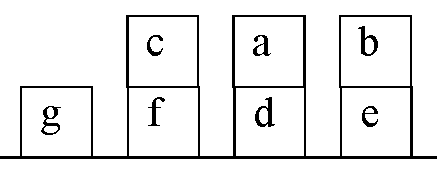
\includegraphics[width=\linewidth]{img/_moving_block_example_green.pdf}
    \end{minipage}\\[0.5em]

    For simplicity, we only consider the action \texttt{MOVE(X, Y, Z)} that moves \texttt{X} from \texttt{Y} to \texttt{Z}.
    It is defined as:
    \[ 
        \begin{split}
            \texttt{clear(X, S)}&, \texttt{clear(Z, S)}, \texttt{on(X, Y, S)}, \texttt{diff(X, Z)} \rightarrow \\
            &\texttt{clear(Y, do(MOVE(X, Y, Z), S))}, \texttt{on(X, Z, do(MOVE(X, Y, Z), S))}
        \end{split}
    \]
    This action can be translated into the following effect axioms:
    \[ 
        \begin{split}
            \lnot\texttt{clear(X, S)} &\vee \lnot\texttt{clear(Z, S)} \vee \lnot\texttt{on(X, Y, S)} \vee \lnot\texttt{diff(X, Z)} \vee \\
            &\texttt{clear(Y, do(MOVE(X, Y, Z), S))}
        \end{split}
    \]
    \[ 
        \begin{split}
            \lnot\texttt{clear(X, S)} &\vee \lnot\texttt{clear(Z, S)} \vee \lnot\texttt{on(X, Y, S)} \vee \lnot\texttt{diff(X, Z)} \vee \\
            &\texttt{on(X, Z, do(MOVE(X, Y, Z), S))}
        \end{split}
    \]
\end{example}

Given the goal \texttt{on(a, b, s1)}, we look for an action whose effects together with $\lnot\texttt{on(a, b, s1)}$ lead to an inconsistency.
We decide to achieve this by using the action \texttt{MOVE(a, Y, b)}, 
therefore making the following substitutions: 
\[ \{ \texttt{X}/\texttt{a}, \texttt{Z}/\texttt{b}, \texttt{s1}/\texttt{do(MOVE(a, Y, b), S)} \} \]
Using the disjunctive formulation (effect axioms), we need to show that the negated preconditions are false
(therefore, making the action applicable):
\begin{center}
    \begin{tabular}{c|c|c|c}
        $\lnot\texttt{clear(a, S)}$ & $\lnot\texttt{clear(b, S)}$ & $\lnot\texttt{on(a, Y, S)}$ & $\lnot\texttt{diff(a, b)}$ \\
        False with $\{ \texttt{S}/\texttt{s0} \}$ & False with $\{ \texttt{S}/\texttt{s0} \}$ 
            & False with $\{ \texttt{S}/\texttt{s0}, \texttt{Y}/\texttt{d} \}$ & False
    \end{tabular}
\end{center}
Therefore, the action \texttt{do(MOVE(a, d, b), s0)} defines the plan to reach the goal \texttt{on(a, b, s1)}.


\subsubsection{Kowalsky's formulation}
\marginnote{Kowalsky's formulation}
Kowalsky's formulation avoids the frame axioms problem by using a set of fixed predicates:
\begin{descriptionlist}
    \item[\texttt{holds(rel, s/a)}] 
        Describes the relations \texttt{rel} that are true in a state \texttt{s} or after the execution of an action \texttt{a}.
    \item[\texttt{poss(s)}]
        Indicates if a state \texttt{s} is possible.
    \item[\texttt{pact(a, s)}]  
        Indicates if an action \texttt{a} can be executed in a state \texttt{s}.
\end{descriptionlist}
Actions can be described as:
\[ \texttt{poss(S)} \land \texttt{pact(A, S)} \rightarrow \texttt{poss(do(A, S))} \]

In Kowalsky's formulation, each action requires a frame assertion (in Green's formulation, each state requires frame axioms).

\begin{example}[Moving blocks]
    An initial state can be described by the following axioms:\\[0.5em]
    \begin{minipage}{.35\linewidth}
        \centering
        \texttt{holds(on(a, b), s0)} \\
        \texttt{holds(ontable(b), s0)} \\
        \texttt{holds(ontable(c), s0)} \\
    \end{minipage}
    \begin{minipage}{.35\linewidth}
        \centering
        \texttt{holds(clear(a), s0)} \\
        \texttt{holds(clear(c), s0)} \\
        \texttt{holds(handempty, s0)} \\
        \texttt{poss(s0)} \\
    \end{minipage}
    \begin{minipage}{.2\linewidth}
        \centering
        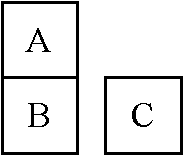
\includegraphics[width=0.6\linewidth]{img/_moving_block_example_kowalsky.pdf}
    \end{minipage}\\[0.5em]
\end{example}

\begin{example}[Moving blocks]
    The action \texttt{UNSTACK(X, Y)} has:
    \begin{descriptionlist}
        \item[Pre-conditions] \texttt{on(X, Y)}, \texttt{clear(X)} and \texttt{handempty}
        \item[Effects] \phantom{}
        \begin{description}
            \item[Add-list] \texttt{holding(X)} and \texttt{clear(Y)}
            \item[Delete-list] \texttt{on(X, Y)}, \texttt{clear(X)} and \texttt{handempty}
        \end{description}
    \end{descriptionlist}

    Its description in Kowalsky's formulation is:
    \begin{descriptionlist}
        \item[Pre-conditions] 
            \[ 
                \begin{split}
                    \texttt{holds(on(X, Y), S)}&, \texttt{holds(clear(X), S)}, \texttt{holds(handempty, S)} \rightarrow \\
                    &\texttt{pact(UNSTACK(X, Y), S)} 
                \end{split}
            \]
        
        \item[Effects] (use add-list)
            \[ \texttt{holds(holding(X), do(UNSTACK(X, Y), S))} \]
            \[ \texttt{holds(clear(Y), do(UNSTACK(X, Y), S))} \]
        
        \item[Frame condition] (uses delete-list)
            \[ 
                \begin{split}
                    \texttt{holds(V, S)}&, \texttt{V} \neq \texttt{on(X, Y)}, \texttt{V} \neq \texttt{clear(X)}, \texttt{V} \neq \texttt{handempty}
                    \rightarrow \\
                    & \texttt{holds(V, do(UNSTACK(X, Y), S))}
                \end{split}
            \]
    \end{descriptionlist}
\end{example}


\subsection{STRIPS}
\marginnote{STRIPS}
STRIPS (Stanford Research Institute Problem Solver) is an ad-hoc algorithm
for linear planning resolution.
The elements of the problem are represented as:
\begin{descriptionlist}
    \item[State] represented with its true fluents.
    \item[Goal] represented with its true fluents.
    \item[Action] represented using three lists:
        \begin{descriptionlist}
            \item[Preconditions] Fluents that are required to be true in order to apply the action.
            \item[Delete-list] Fluents that become false after the action.
            \item[Add-list] Fluents that become true after the action.
        \end{descriptionlist}
        Add-list and delete-list can be combined in an effect list with positive (add-list) and negative (delete-list) axioms.

        \begin{description}
            \item[STRIPS assumption] Everything that is not in the add-list or delete-list is unchanged in the next state. 
        \end{description}
\end{descriptionlist}

STRIPS uses two data structures:
\begin{descriptionlist}
    \item[Goal stack] Does a backward search to reach the initial state.
    \item[Current state] Represents the forward application of the actions found using the goal stack.
\end{descriptionlist}

\begin{algorithm}[H]
\caption{STRIPS}
\begin{lstlisting}[mathescape=true]
def strips(problem):
    goal_stack = Stack()
    current_state = State(problem.initial_state)
    goal_stack.push(problem.goal)
    plan = []
    while not goal_stack.empty():
        if (goal_stack.top() is a single/conjunction of goals and
            there is a substitution $\theta$ that makes it $\subseteq$ current_state):
            A = goal_stack.pop()
            $\theta$ = find_substitution(A, current_state)
            goal_stack.apply_substitution($\theta$)
        elif goal_stack.top() is a single goal:
            R = rule with a $\in$ R.add_list
            _ = goal_stack.pop() # Pop goal
            goal_stack.push(R)
            goal_stack.push(R.preconditions)
        elif goal_stack.top() is a conjunction of goals:
            for g in permutation(goal_stack.top()):
                goal_stack.push(g)
            # Note that there is no pop
        elif goal_stack.top() is an action:
            action = goal_stack.pop()
            current_state.apply(action)
            plan.append(action)
    return plan
\end{lstlisting}
\end{algorithm}

\begin{example}[Moving blocks] 
    \begin{center}
        
\includegraphics[width=0.85\textwidth]{img/_strips_example1.pdf}
        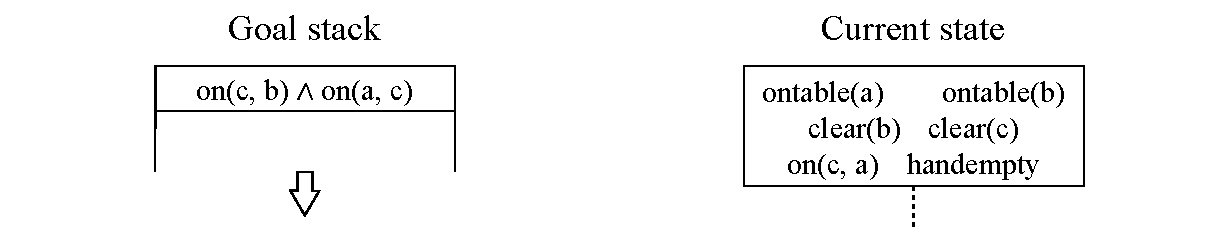
\includegraphics[width=0.85\textwidth]{img/_strips_example2.pdf}
        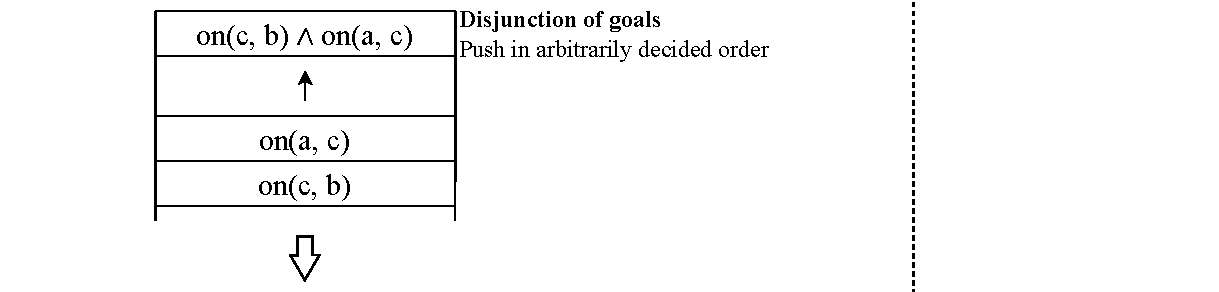
\includegraphics[width=0.85\textwidth]{img/_strips_example3.pdf}
        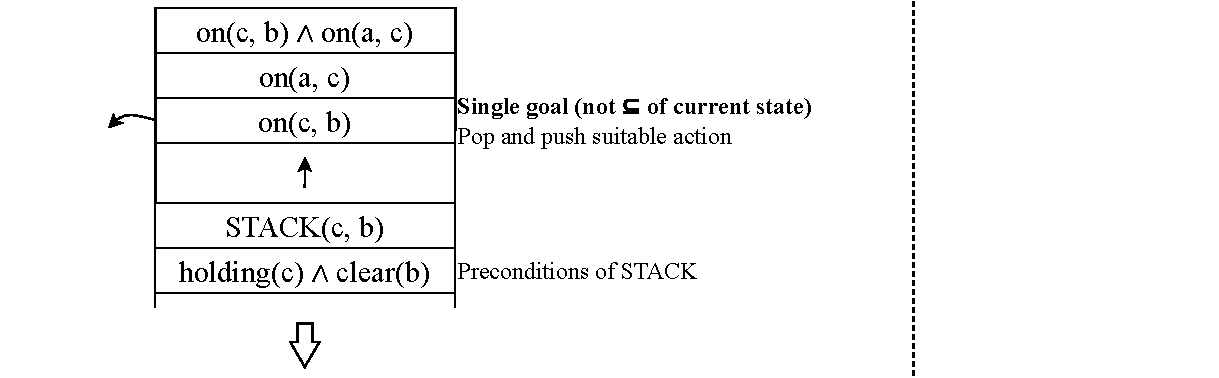
\includegraphics[width=0.85\textwidth]{img/_strips_example4.pdf}
        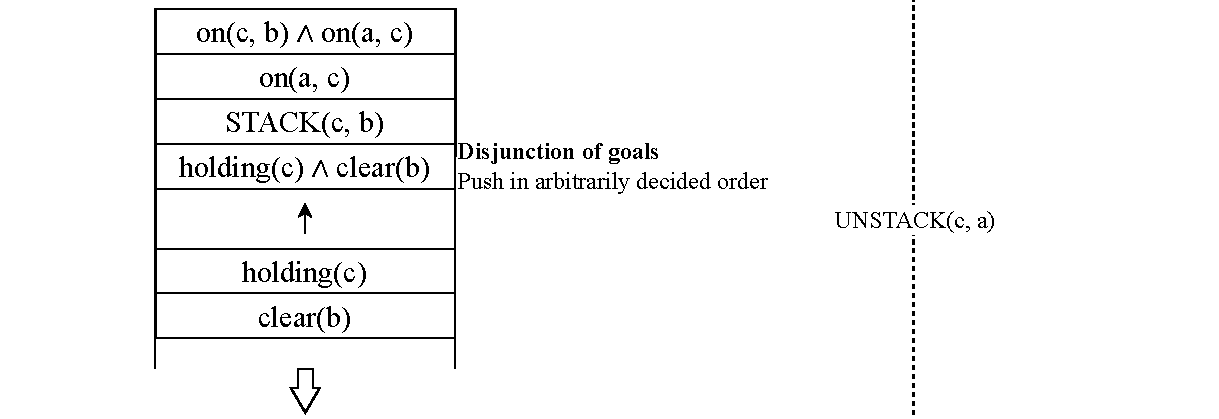
\includegraphics[width=0.85\textwidth]{img/_strips_example5.pdf}
        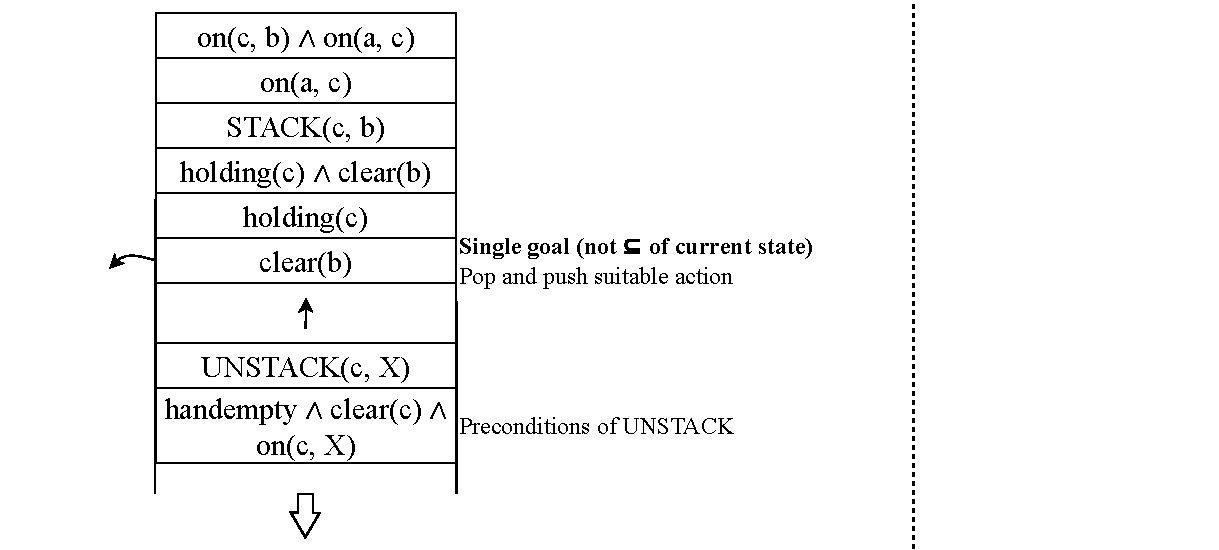
\includegraphics[width=0.85\textwidth]{img/_strips_example6.pdf}
        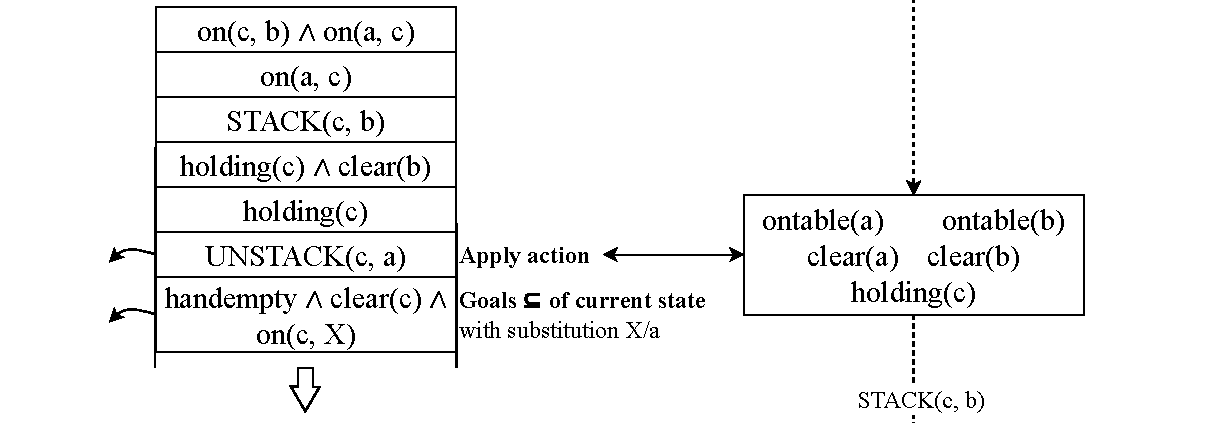
\includegraphics[width=0.85\textwidth]{img/_strips_example7.pdf}
        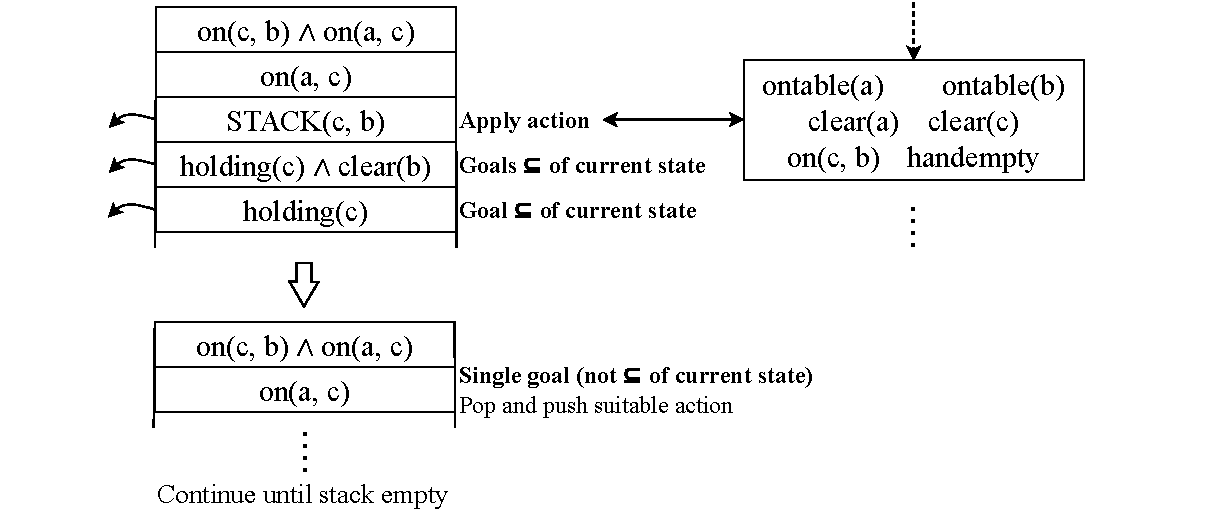
\includegraphics[width=0.85\textwidth]{img/_strips_example8.pdf}
    \end{center}
\end{example}

Since there are non-deterministic choices, the search space might become very large.
Heuristics can be used to avoid this.

Conjunction of goals is solved separately, but this can lead to the \marginnote{Sussman anomaly} \textbf{Sussman anomaly} 
where a sub-goal destroys what another sub-goal has done.
For this reason, when a conjunction is encountered, it is not immediately popped from the goal stack
and is left as a final check.



\section{Non-linear planning}
\marginnote{Non-linear planning}


\subsection{Partial order planning}

Non-linear planning finds a plan as a search problem in the space of plans (instead of states as in linear planning).
Each node of the search tree is a partial plan. Edges represent plan refinement operations.

A non-linear plan is represented by:
\begin{descriptionlist}
    \item[Actions{\normalfont.}] \marginnote{Actions set}
    \item[Orderings] \marginnote{Orderings set}
        between actions.
    \item[Causal links] \marginnote{Causal links}
        triplet $\langle S_i, S_j, c \rangle$ where $S_i$ and $S_j$ are actions and $c$ is a sub-goal.
        $c$ should be in the effects of $S_i$ and in the preconditions of $S_j$.

        Causal links represent causal relations between actions (i.e. interaction between sub-goals): 
        to execute $S_j$, the effect $c$ of $S_i$ is required first.
\end{descriptionlist}

The initial plan is an empty plan with two fake actions \texttt{start} and \texttt{stop} 
with ordering $\texttt{start} < \texttt{stop}$:
\begin{descriptionlist}
    \item[\texttt{start}] has no preconditions and the effects match the initial state.
    \item[\texttt{stop}] has no effects and the preconditions match the goal.
\end{descriptionlist}
At each step, one of the following refinement operations can be applied until the goal is reached:
\begin{itemize}
    \item Add an action to the set of actions.
    \item Add an ordering to the set of orderings.
    \item Add a causal link to the set of causal links.
\end{itemize}

\begin{figure}[H]
    \centering
    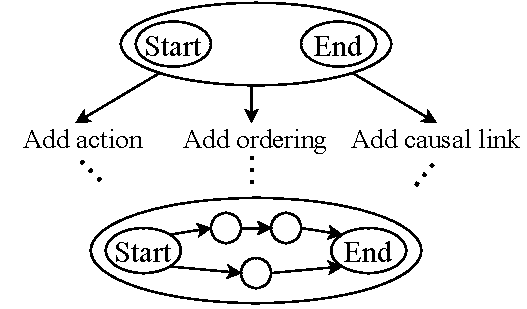
\includegraphics[width=0.45\textwidth]{img/_nonlinear_plan_example.pdf}
    \caption{Example of search tree in non-linear planning}
\end{figure}


\begin{description}
    \item[Least commitment planning] \marginnote{Least commitment planning}
        Only strictly necessary restrictions (e.g. ordering) are imposed.
        Non-linear planning is a least commitment planning.

    \item[Linearization] \marginnote{Linearization} 
        At the end, the partially ordered actions should be linearized, 
        respecting the ordering constraints, to obtain the final plan.
\end{description}


\begin{description}
    \item[Threat] \marginnote{Threat} 
        An action $S_k$ is a threat to a causal link $\langle S_i, S_j, c \rangle$ 
        if its effects cancel $c$.
        $S_k$ should not be executed in between $S_i$ and $S_j$.

        \begin{figure}[H]
            \centering
            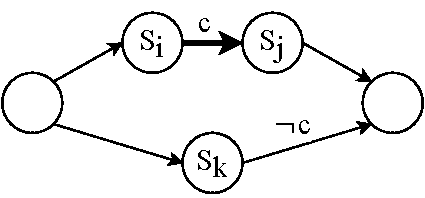
\includegraphics[width=0.3\textwidth]{img/_threat_example.pdf}
            \caption{Example of threat. Causal links are represented using thick arrows.}
        \end{figure}

        Possible solutions to a threat $S_k$ to $\langle S_i, S_j, c \rangle$ are:
        \begin{descriptionlist}
            \item[Demotion] \marginnote{Demotion}
                Add the ordering constraint $S_k < S_i$ (i.e. threat executed before).
            \item[Promotion] \marginnote{Promotion}
                Add the ordering constraint $S_k > S_j$ (i.e. threat executed after).
        \end{descriptionlist}
\end{description}

\begin{algorithm}[H]
\caption{Partial order planning (POP)}
\begin{lstlisting}[mathescape=true]
def pop(initial_state, goal, actions):
    plan = init_empty_plan(initial_state, goal)
    while not plan.isSolution():
        try:
            sn, c = selectSubgoal(plan)
            chooseOperator(plan, actions, sn, c)
            resolveThreats(plan)
        except PlanFailError:
            plan.backtrack()
    return plan

def selectSubgoal(plan):
    sn, c = random([sn, c in plan.steps if c in sn.unsolved_preconditions])
    return sn, c

def chooseOperator(plan, actions, sn, c):
    s = random([s in (actions + plan.steps) if c in s.effects])
    if s is None: raise(PlanFailError)
    plan.addCausalLink($\langle$s, sn, c$\rangle$)
    plan.addOrdering(s < sn)
    if s not in plan.steps:
        plan.addAction(s)
        plan.addOrdering(start < s < stop)

def resolveThreats(plan):
    for s_k, s_i, s_j in plan.threats():
        resolution = random([ DEMOTION, PROMOTION ])
        if resolution == DEMOTION:
            plan.addOrdering(s_k < s_i)
        elif resolution == PROMOTION:
            plan.addOrdering(s_k > s_j)
        if plan.isNotConsistent(): raise(PlanFailError)
\end{lstlisting}
\end{algorithm}

\begin{example}[Purchasing schedule]
    The initial state is: 
    \[ \texttt{at(home)}, \texttt{sells(hws, drill)}, \texttt{sells(sm, milk)}, \texttt{sells(sm, banana)} \]
    where $\texttt{hws}$ means "hardware store" and $\texttt{sm}$ means "supermarket".
    
    The goal is:
    \[ \texttt{at(home)}, \texttt{have(drill)}, \texttt{have(milk)}, \texttt{have(banana)} \]

    The possible actions are:\\[0.5em]
    \begin{minipage}{.5\linewidth}
        \begin{descriptionlist}
            \item[\texttt{GO(X, Y)}] \phantom{}
                \begin{description}
                    \item[Preconditions] $\texttt{at(X)}$
                    \item[Effects] $\texttt{at(Y)}$, $\lnot \texttt{at(X)}$
                \end{description}
        \end{descriptionlist}
    \end{minipage}
    \begin{minipage}{.5\linewidth}
        \begin{descriptionlist}
            \item[\texttt{BUY(S, Y)}] \phantom{}
            \begin{description}
                \item[Preconditions] $\texttt{at(S)}$, $\texttt{sells(S, Y)}$
                \item[Effects] $\texttt{have(Y)}$
            \end{description}
        \end{descriptionlist}
    \end{minipage}\\[0.5em]

    Partial order planning steps are:
    \begin{enumerate}
        \item Define the initial plan:
            \begin{center}
                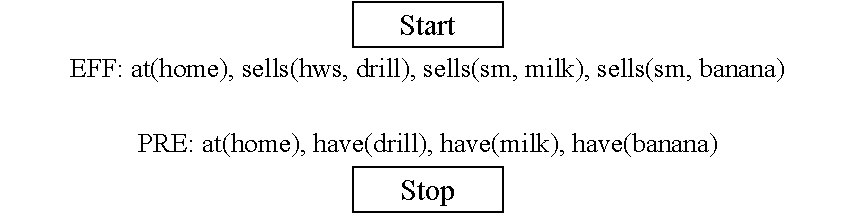
\includegraphics[width=0.7\textwidth]{img/_pop_example1.pdf}
            \end{center}

        \item The loop of POP is:
            \begin{itemize}
                \item Choose an action $a_i$ and one of its unsolved preconditions $c$. 
                \item Select an action $a_j$ with the precondition $c$ in its effects.
                \item Add the ordering constraint $\texttt{start} < a_j < \texttt{stop}$.
                \item Add the causal link $\langle a_j, a_i, c \rangle$ (and ordering $a_j < a_i$).
                \item Solve threats.
            \end{itemize}
        
            We choose the action $a_i = \texttt{stop}$ and the precondition $c = \texttt{have(drill)}$.
            We choose as action with $c$ in its effects $a_j = \texttt{BUY(X, drill)}$.
            We therefore add to the plan the ordering $\texttt{start} < \texttt{BUY(X, drill)} < \texttt{stop}$ and
            the causal link $\langle \texttt{BUY(X, drill)}, \texttt{stop}, \texttt{have(drill)} \rangle$:
            \begin{center}
                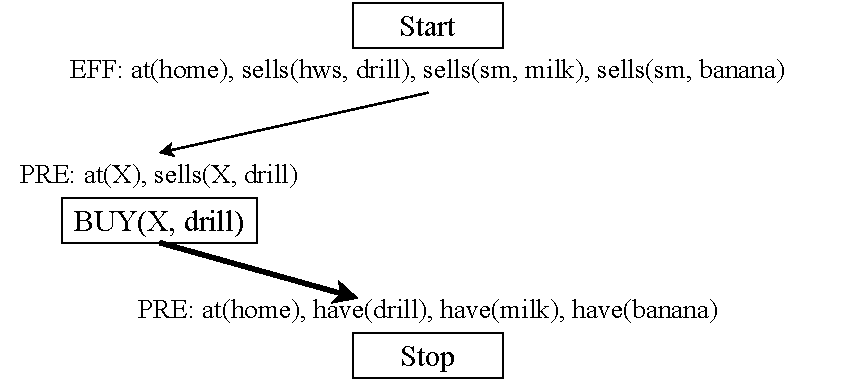
\includegraphics[width=0.7\textwidth]{img/_pop_example2.pdf}
            \end{center}

        \item Repeat the previous point for the preconditions $\texttt{have(milk)}$ and $\texttt{have(banana)}$:
            \begin{center}
                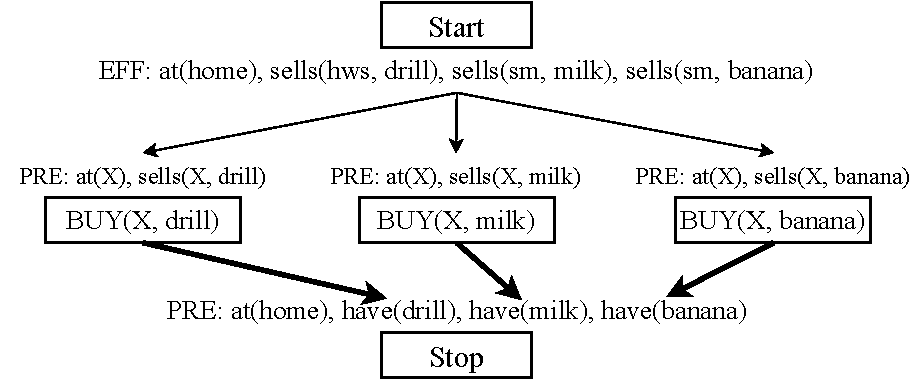
\includegraphics[width=0.7\textwidth]{img/_pop_example3.pdf}
            \end{center}

        \item Now, we choose as action $\texttt{BUY(X, drill)}$ and as unsolved precondition $\texttt{sells(X, drill)}$.
            This can be solved from the action $\texttt{start}$ with effect $\texttt{sells(hws, drill)}$.
            We make the substitution $\texttt{X}/\texttt{hws}$ and 
            add $\langle \texttt{start}, \texttt{BUY(hws, drill)}, \texttt{sells(hws, drill)} \rangle$ to the causal links.
            The same process can be repeated for $\texttt{BUY(X, milk)}$ and $\texttt{BUY(X, banana)}$:
            \begin{center}
                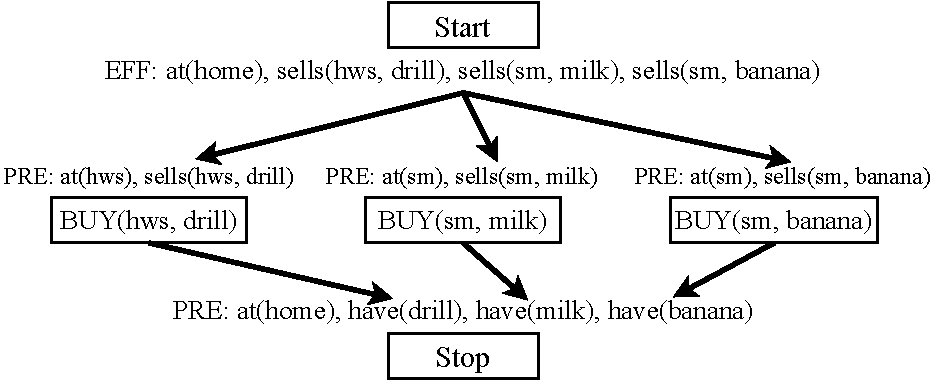
\includegraphics[width=0.7\textwidth]{img/_pop_example4.pdf}
            \end{center}

        \item Now, we choose as action $\texttt{BUY(hws, drill)}$ and as unsolved precondition $\texttt{at(hws)}$.
            This can be solved using the action $\texttt{GO(X, hws)}$.
            We add $\langle \texttt{GO(X, hws)}, \texttt{BUY(hws, drill)}, \texttt{at(hws)} \rangle$ to the causal links.

            We continue by choosing as action $\texttt{GO(X, hws)}$ and as unsolved precondition $\texttt{at(X)}$.
            This can be solved from $\texttt{start}$ with effect $\texttt{at(home)}$.
            We therefore make the substitution $\texttt{X}/\texttt{home}$ and 
            add $\langle \texttt{start}, \texttt{GO(home, hws)}, \texttt{at(home)} \rangle$ to the causal links.

            The same process can be repeated for the $\texttt{milk}$ and $\texttt{banana}$ branch:
            \begin{center}
                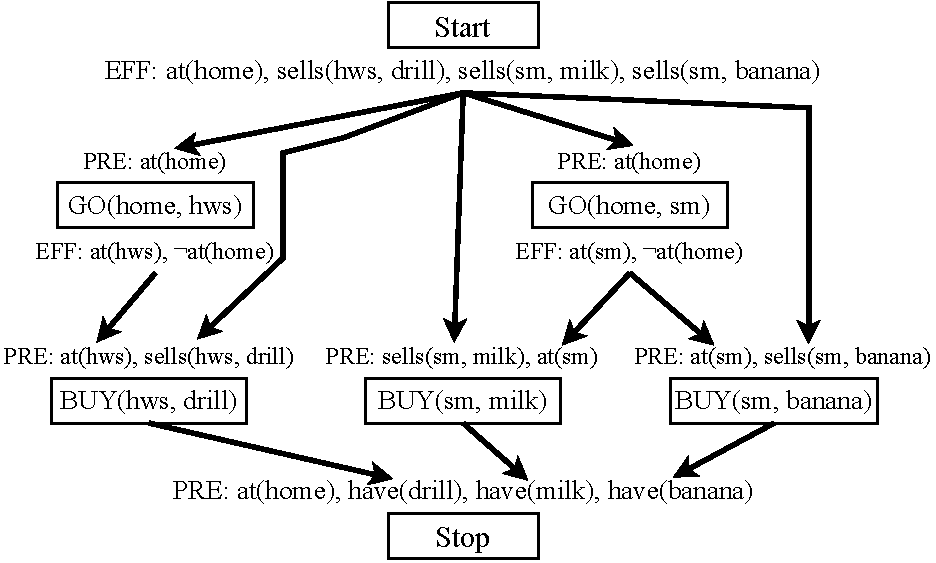
\includegraphics[width=0.7\textwidth]{img/_pop_example5.pdf}
            \end{center}

        \item We have a threat between $\texttt{GO(home, hws)}$ and $\texttt{GO(home, sm)}$ as they both
            require the precondition $\texttt{at(home)}$ and both have as effect $\lnot\texttt{at(home)}$.
            It can be easily seen that neither promotion nor demotion solves the conflict. 
            We are therefore forced to backtrack.

            We backtrack at the previous point, where we chose as action $\texttt{GO(X, sm)}$ and as precondition $\texttt{at(X)}$
            (this step has been implicitly done in the previous point).
            \begin{itemize}
                \item Instead of choosing the action $\texttt{start}$, we choose $\texttt{GO(home, hws)}$ with the effect $\texttt{at(hws)}$.
                    We therefore make the substitution $\texttt{X}/\texttt{hws}$ and update the causal links.
                \item We also resolve the threat $\texttt{GO(hws, sm)}$ to $\texttt{BUY(hws, drill)}$
                    (it removes the precondition $\texttt{at(hws)}$)
                    by promoting $\texttt{GO(hws, sm)}$
                    and adding the ordering constraint $\texttt{BUY(hws, drill)} < \texttt{GO(hws, sm)}$:
            \end{itemize}
            \begin{center}
                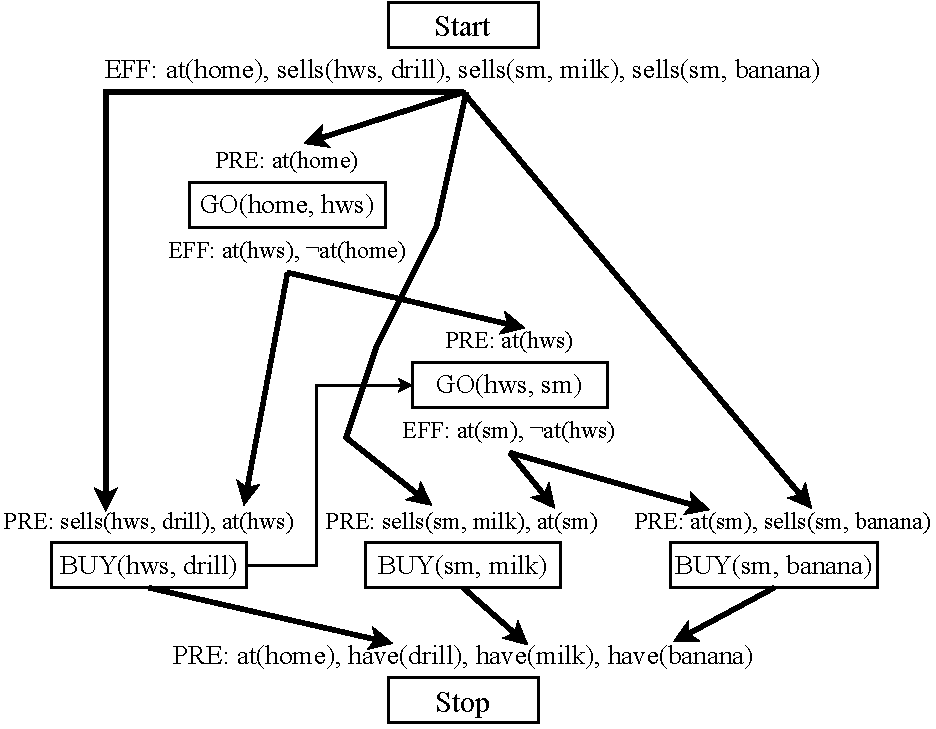
\includegraphics[width=0.7\textwidth]{img/_pop_example6.pdf}
            \end{center}

        \item Now, we choose as action $\texttt{stop}$ and as precondition $\texttt{at(home)}$.
            We choose as action $\texttt{GO(sm, home)}$ and update the causal links.
            
            Finally, we solve the threat $\texttt{GO(sm, home)}$ to 
            both $\texttt{BUY(sm, milk)}$ and $\texttt{BUY(sm, banana)}$ (it removes the required precondition $\texttt{at(sm)}$)
            by promoting $\texttt{GO(sm, home)}$.
            The newly added ordering constraints are 
            $\texttt{BUY(sm, milk)} < \texttt{GO(sm, home)}$ and 
            $\texttt{BUY(sm, banana)} < \texttt{GO(sm, home)}$.
            
            The final plan is:
            \begin{center}
                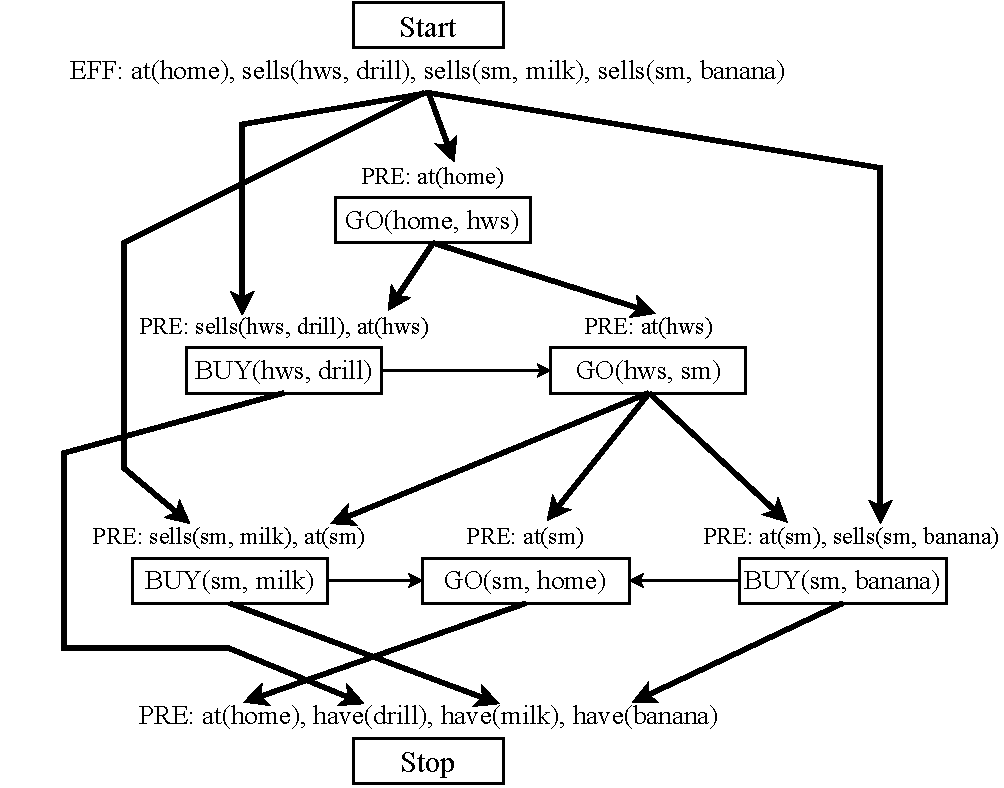
\includegraphics[width=0.7\textwidth]{img/_pop_example7.pdf}
            \end{center}
            By considering the ordering constraints, a linearization could be:
            \[ 
                \begin{split}
                    \texttt{GO(home, hws)} &\rightarrow  
                    \texttt{BUY(hws, drill)} \rightarrow  
                    \texttt{GO(hws, sm)} \rightarrow\\
                    &\texttt{BUY(sm, milk)} \rightarrow  
                    \texttt{BUY(sm, banana)} \rightarrow  
                    \texttt{GO(sm, home)} 
                \end{split}
            \]
    \end{enumerate}
\end{example}


\subsection{Modal truth criterion}
\marginnote{Modal truth criterion}

Modal truth criterion uses five plan refinement methods that 
ensures the completeness of the planner (POP is not complete).

MTC refinement methods are:
\begin{descriptionlist}
    \item[Establishment] \marginnote{Establishment}
        The same standard operations of POP:
        \begin{enumerate}
            \item Insert a new action in the plan.
            \item Add an ordering constraint.
            \item Do a variable assignment.
        \end{enumerate}

    \item[Promotion] \marginnote{Promotion}
        As in POP.

    \item[Demotion] \marginnote{Demotion}
        As in POP.

    \item[White knight] \marginnote{White knight}
        Insert an operator $S_n$ between $S_k$ and $S_j$, where $S_k$ threatens $S_j$,
        in such way that $S_n$ re-establishes the preconditions of $S_j$.

    \item[Separation] \marginnote{Separation}
        Add a constraint to a variable to avoid that it unifies with an unwanted value.
\end{descriptionlist}



\section{Hierarchical planning}
\marginnote{Hierarchical planning}
Hierarchical planning allows to create a complex plan at different levels of abstraction.
Different meta-level searches are executed to generate meta-level plans that are progressively refined.


\subsection{ABSTRIPS}
\marginnote{ABSTRIPS}
In ABSTRIPS, a criticality value is assigned to each precondition based on the complexity of its achievement.

At each level, a plan is found assuming that the preconditions corresponding to lower levels of criticality are true
(i.e. solve harder goals first).
At the next level, the previously found plan and its preconditions are used as starting point in the goal stack.

\begin{algorithm}
\caption{ABSTRIPS}
\begin{lstlisting}[mathescape=true]
    def abstrips(problem, start_threshold, threshold_step):
        threshold = start_threshold
        plan = None
        while $\text{there is a precondition still not considered}$:
            true_preconds = problem.preconds[criticality < threshold]
            plan = strips(problem, true_preconds, starting_plan=plan)
            threshold -= threshold_step
        return plan
\end{lstlisting}
\end{algorithm}



\subsection{Macro-operators}
\marginnote{Macro-operators}
In macro-operators, two types of operators are defined:
\begin{descriptionlist}
    \item[Atomic] Elementary operations that can be executed by an agent.
    \item[Macro] Set of atomic operators. Before execution, this type of operator has to be decomposed.
        \begin{description}
            \item[Precompiled decomposition] 
                The decomposition is known and described alongside the preconditions and effects of the operator.
            \item[Planned decomposition] 
                The planner has to synthesize the atomic operators that compose a macro operator.
        \end{description}

        Constraints are needed for a safe decomposition.
        Let $A$ be a macro with effect $X$ and $P$ its decomposition:
        \begin{itemize}
            \item $X$ must be the effect of at least an atomic action in $P$ and should be protected until the end of $P$.
            \item Each precondition of the actions in $P$ must be guaranteed by previous actions or be a precondition of $A$.
            \item $P$ must not threaten any causal link.
        \end{itemize}

        Moreover, when a macro action $A$ is replaced with its decomposition $P$:
        \begin{itemize}
            \item For each $B$ such that $B < A$, impose the ordering $B < \texttt{First($P$)}$.
            \item For each $B$ such that $A < B$, impose the ordering $\texttt{Last($P$)} < B$.
            \item Each causal link $\langle S, A, c \rangle$ is replaced with $\langle S, S_i, c \rangle$,
                where $S_i$ are actions in $P$ with precondition $c$ and do not have other atomic operators of the macro before.
            \item Each causal link $\langle A, S, c \rangle$ is replaced with $\langle S_i, A, c \rangle$,
                where $S_i$ are actions in $P$ with effect $c$ and do not have other atomic operators of the macro after.
        \end{itemize}
        
\end{descriptionlist}

\begin{algorithm}
\caption{Hierarchical decomposition POP}
\begin{lstlisting}[mathescape=true]
def hdpop(initial_state, goal, actions, decomposition_methods):
    plan = init_empty_plan(initial_state, goal)
    while not plan.isSolution():
        try:
            if choice() == ESTABLISHMENT:
                sn, c = selectSubgoal(plan)
                chooseOperator(plan, actions, sn, c)
            else:
                macro = selectMacroStep(plan)
                chooseDecomposition(macro, decomposition_methods, plan)
            resolveThreats(plan)
        except PlanFailError:
            plan.backtrack()
    return plan
\end{lstlisting}
\end{algorithm}



\section{Conditional planning}
\marginnote{Conditional planning}
Conditional planning is based on the open-world assumption where what is not in the initial state is unknown.
It generates a different plan for each source of uncertainty and therefore has exponential complexity.

\begin{description}
    \item[Sensing action] 
        Action with pre-conditions and post-conditions that allows to obtain unknown information.
\end{description}


\begin{example}[Inflate tire]
    \phantom{}\\
    \begin{center}
        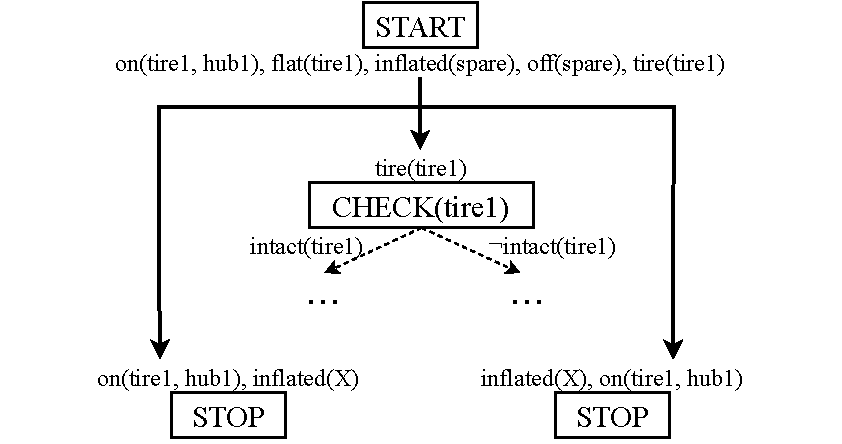
\includegraphics[width=0.65\textwidth]{img/_conditional_planning.pdf}
    \end{center}

    When executing a sensing action (\texttt{CHECK(tire1)}), a copy of the goal is generated for each possible scenario.
\end{example}



\section{Reactive planning}
Reactive planners are online algorithms able to interact with the dynamicity of the world.

\subsection{Pure reactive systems}
\marginnote{Pure reactive systems}
Pure reactive planners have a knowledge base that describes the conditions for which an action has to be executed.
The choice of the action is predictable. Therefore, this approach is not suited for domains that require reasoning.

\subsection{Hybrid systems}
\marginnote{Hybrid systems}
Hybrid planners integrate the generative and reactive approaches.
The steps the algorithm does are:
\begin{itemize}
    \item Generates a plan to achieve the goal.
    \item Checks the pre-conditions and post-conditions of the action it is going to execute.
    \item Backtracks the effects of an action in case of a failure.
    \item Corrects the plan if external events occur.
\end{itemize}



\section{Graphplan}
\marginnote{Graphplan}
Graphplan is an off-line, least-commitment, closed-world planner that
constructs a partially ordered set of actions through a planning graph based on time steps.

The planner is correct, complete, optimal and computationally efficient.


\begin{description}
    \item[Action] \marginnote{Actions}
        An action, as in STRIPS, has:
        \begin{itemize}
            \item Preconditions.
            \item Add list.
            \item Delete list.
        \end{itemize}

        \begin{description}
            \item[\texttt{NO-OP}] 
                Action that does not change the state (to solve the frame problem).
                Can be seen as an action with the same proposition as precondition and add list.
        \end{description}

    \item[State] \marginnote{State}
        A state is represented by a set of propositions that are true in that time step.

    \item[Planning graph] \marginnote{Planning graph}
        Directed leveled graph where edges connect nodes of adjacent levels.

        There are two possible levels that are alternated during construction:
        \begin{descriptionlist}
            \item[Proposition level] 
                Contains propositions that describe the state. 
                Note that interfering propositions can appear.
            \item[Action level] 
                Contains all the possible actions that have as preconditions the propositions in the previous level.
                Note that interfering actions can appear.
        \end{descriptionlist}
        The first level of the graph is a proposition level containing the initial state.

        Edges can be:
        \begin{descriptionlist}
            \item[Precondition arcs] proposition $\rightarrow$ action.
            \item[Add arcs] action $\rightarrow$ proposition.
            \item[Delete arcs] action $\rightarrow$ proposition.
        \end{descriptionlist}

    \item[Inconsistency] \marginnote{Inconsistency}
        Actions and propositions in the same time step can be inconsistent.
        Possible causes are:
        \begin{descriptionlist}
            \item[Actions] \phantom{}
                \begin{description}
                    \item[Inconsistent effects] \marginnote{Inconsistent effects}
                        An action negates the effects of another one.
                    
                    \item[Interference] \marginnote{Interference}
                        An action deletes the preconditions of another one.
                
                    \item[Competing needs] \marginnote{Competing needs} 
                        Two actions have mutually exclusive preconditions.
        
                    \item[Domain dependent] 
                \end{description}

            \item[Propositions] \marginnote{Inconsistent propositions}
                Propositions are inconsistent when they cannot appear together either 
                because one negates the other or
                because they can be reached only through mutually exclusive paths.
        \end{descriptionlist}

    \item[Plan extraction] \marginnote{Plan extraction}
        Once a proposition level containing the goal as non-mutually exclusive propositions has been reached,
        the algorithm can attempt to extract a plan.
        A valid plan has the following properties:
        \begin{itemize}
            \item Actions in the same time step do not interfere and can be executed in any order.
            \item Propositions at the same time step are non-mutually exclusive.
            \item The last step contains the goal as non-mutually exclusive propositions.
        \end{itemize}
        Even if the last step is a superset of the goal, planning may still fail.
        In this case, the algorithm has to continue generating levels.
        % Loop detection can be used to stop when a plan cannot be found.

    \item[Memoization] \marginnote{Memoization}
        At each step, if the goal is not satisfiable, the result is saved and 
        when the same state is encountered in the future it will automatically fail.
\end{description}


\begin{theorem}
    The following statements hold:
    \begin{itemize}
        \item If a valid plan exists, it can be found as a subgraph of the planning graph.
        
        \item In a planning graph, two actions in a time step are mutually exclusive
            if a valid plan containing both does not exist.

        \item In a planning graph, two propositions are mutually exclusive if they are inconsistent.
    \end{itemize}
\end{theorem}

\begin{corollary}
    Inconsistencies found during the planning graph construction
    prune paths in the search tree.
\end{corollary}


\begin{algorithm}[H]
\caption{Graphplan}
\begin{lstlisting}[mathescape=true]
def graphplan(initial_state, actions, goal):
    graph = PlanningGraph()
    graph.addPropositionLevel(initial_state)
    while True:
        if (goal in graph.lastPropositionLevel and 
            not mutexPropositions(goal, graph.lastPropositionLevel)):
            plan = extractSolution(graph, goal)
            if plan is not FAIL: return plan
        graph.addActionLevel( selectActions(graph) )
        graph.addPropositionLevel( selectPreconditions(graph, actions) )

def selectActions(graph, actions):
    new_action_level = Level()
    for action in actions.unify(graph.lastPropositionLevel):
        preconds = action.preconditions
        if not mutexPropositions(preconds, graph.lastPropositionLevel):
            new_action_level.add(preconds, action)
    for proposition in graph.lastPropositionLevel:
        new_action_level.add(NO_OP(proposition))
    new_action_level.findInconsistencies()
    return new_action_level

def selectPreconditions(graph):
    new_props_level = Level()
    for action in graph.lastActionLevel:
        for prop in action.add_list:
            new_props_level.add(action, prop, "add")
        for prop in action.delete_list:
            new_props_level.add(action, prop, "delete")
    new_props_level.findInconsistencies()
    return new_props_level

def extractSolution(graph, goal):
    plan = Plan()
    actions = graph.lastActionLevel.getActionsWithEffect(goal)
    if mutexActions(actions, graph.lastActionLevel): return FAIL
    plan.addLevel(actions)
    graph = graph.popLastActionLevel()
    return plan.merge(extractSolution(graph, actions.preconditions))
\end{lstlisting}
\end{algorithm}


\begin{example}[Moving objects with a cart]
    Given the actions:
    \begin{descriptionlist}
        \item[\texttt{MOVE(R, PosA, PosB)}] \phantom{}
            \begin{description}
                \item[Preconditions] $\texttt{at(R, PosA)}$, $\texttt{hasFuel(R)}$
                \item[Add list] $\texttt{at(R, PosB)}$
                \item[Delete list] $\texttt{at(R, PosA)}$, $\texttt{hasFuel(R)}$
            \end{description}
    \end{descriptionlist}

    \begin{minipage}{0.5\textwidth}
        \begin{descriptionlist}
            \item[\texttt{LOAD(Obj, Pos)}] \phantom{}
                \begin{description}
                    \item[Preconds] $\texttt{at(R, Pos)}$, $\texttt{at(Obj, Pos)}$
                    \item[Add list] $\texttt{in(R, Obj)}$
                    \item[Delete list] $\texttt{at(Obj, Pos)}$
                \end{description}
        \end{descriptionlist}
    \end{minipage}
    \begin{minipage}{0.5\textwidth}
        \begin{descriptionlist}
            \item[\texttt{UNLOAD(Obj, Pos)}] \phantom{}
                \begin{description}
                    \item[Preconds] $\texttt{in(R, Obj)}$, $\texttt{at(R, Pos)}$
                    \item[Add list] $\texttt{at(Obj, Pos)}$
                    \item[Delete list] $\texttt{in(R, Obj)}$
                \end{description}
        \end{descriptionlist}
    \end{minipage}

    Given a scenario where:
    \begin{itemize}
        \item \texttt{r} is a cart.
        \item \texttt{a} and \texttt{b} are objects.
        \item \texttt{l} and \texttt{p} are locations.
    \end{itemize}
    and the initial state:
    \begin{center}
        \texttt{at(a, l)} $\cdot$ \texttt{at(b, l)} $\cdot$ \texttt{at(r, l)} $\cdot$ \texttt{hasFuel(r)} 
    \end{center}

    The first four time steps of the planning graph are:
    \begin{center}
        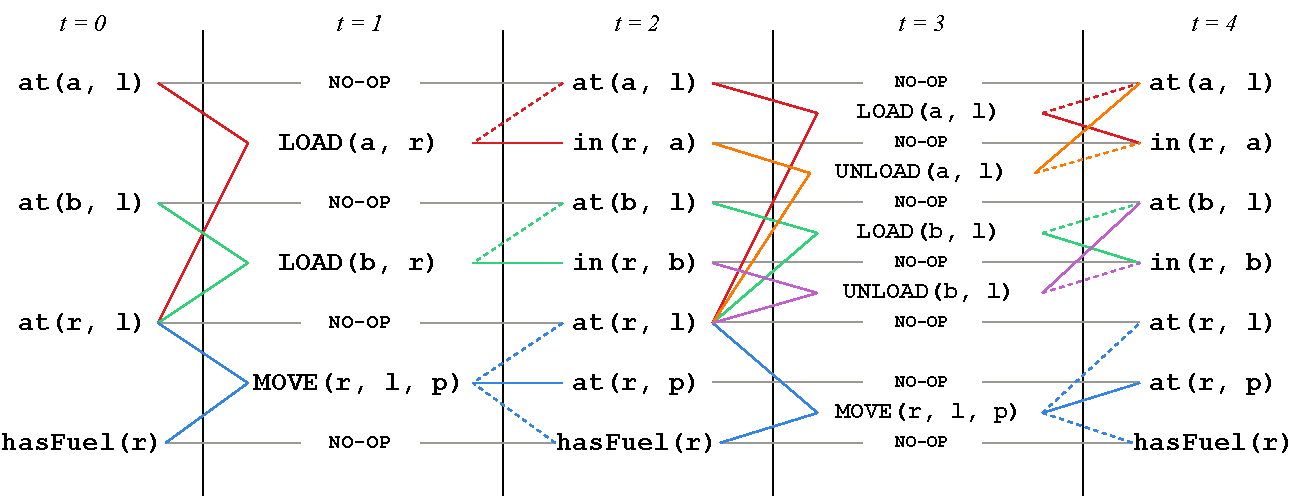
\includegraphics[width=\textwidth]{img/_graphplan.pdf}
    \end{center}

    The inconsistencies at $t=1$ are:
    \begin{descriptionlist}
        \item[Inconsistent effects] \phantom{}\\[0.5em]
            $\begin{cases}\texttt{NO-OP} \\ \texttt{LOAD(a, r)}\end{cases} \text{for } \texttt{at(a, l)}$,
            $\begin{cases}\texttt{NO-OP} \\ \texttt{LOAD(b, r)}\end{cases} \text{for } \texttt{at(b, l)}$,\\[0.3em]
            $\begin{cases}\texttt{NO-OP} \\ \texttt{MOVE(r, l, p)}\end{cases} \text{for } \texttt{at(r, l)}$,
            $\begin{cases}\texttt{NO-OP} \\ \texttt{MOVE(r, l, p)}\end{cases} \text{for } \texttt{hasFuel(r)}$

        \item[Interference] \phantom{}\\[0.5em]
            $\begin{cases}\texttt{MOVE(r, l, p)} \\ \texttt{LOAD(a, r)}\end{cases} \text{for } \texttt{at(r, l)}$,
            $\begin{cases}\texttt{MOVE(r, l, p)} \\ \texttt{LOAD(b, r)}\end{cases} \text{for } \texttt{at(r, l)}$
    \end{descriptionlist}

    The inconsistencies of propositions at $t=2$ are:
    \begin{itemize}
        \item Consequence of the add and delete list of each action:\\[0.3em]
            $\begin{cases}\texttt{at(a, l)} \\ \texttt{in(r, a)}\end{cases}$,
            $\begin{cases}\texttt{at(b, l)} \\ \texttt{in(r, b)}\end{cases}$,
            $\begin{cases}\texttt{at(r, l)} \\ \texttt{at(r, p)}\end{cases}$,
            $\begin{cases}\texttt{at(r, p)} \\ \texttt{hasFuel(r)}\end{cases}$\\[0.5em]
        \item Consequence of the add list of interfering actions (mutual exclusion):\\[0.3em]
            $\begin{cases}\texttt{in(r, a)} \\ \texttt{at(r, p)}\end{cases}$,
            $\begin{cases}\texttt{in(r, b)} \\ \texttt{at(r, p)}\end{cases}$
    \end{itemize}

    Note that because of the mutually exclusive propositions at $t=2$, 
    at $t=3$ the actions \texttt{UNLOAD($\cdot$, p)} cannot be performed.
\end{example}


\subsection{Fast forward}
\marginnote{Fast forward}
Heuristic planner based on Graphplan, hill climbing and A$^*$.

\begin{description}
    \item[Heuristic]
        Given a problem $P$, the algorithm considers a relaxation $P^+$ 
        where delete effects are ignored.
        $P^+$ is solved using Graphplan and the number of actions required to solve it is used as lower bound heuristic for $P$.

    \item[Algorithm] \phantom{}
        \begin{enumerate}
            \item From a state $S$, examine the successors.
            \item If there is a successor $S'$ better than $S$, move into it and return to point 1.
            \item Otherwise, run a complete A$^*$ search.
        \end{enumerate}
\end{description}
